\clearpage
\begin{examplebox}
	\textbf{\textcolor{CExample}{例 1（基础）}}
\begin{center}\begin{tikzpicture}[font=\small,>=stealth,line join=round]
\draw[gray!40,rounded corners=3pt] (0,0) rectangle (14.2,8.3);
\node[text width=12.6cm,align=center] at (7.1,7.65) {关于 $x$ 轴：同一横坐标，上下高度相反};
\begin{scope}[shift={(4.3,4.1)},x=1.65cm,y=0.47000000000000003cm]
\draw[->,gray] (-2,0)--(2,0) node[right]{$x$};\draw[->,gray] (0,-5)--(0,5) node[above]{$y$};

\begin{scope}\clip (-2,-5) rectangle (2,5);
\draw[blue,thick,domain=-2:2,samples=180] plot(\x,{3*\x+2});
\draw[orange!85!black,thick,domain=-2:2,samples=180] plot(\x,{-3*\x-2});
\end{scope}
\fill[blue] (0,2) circle(2.2pt);\node[above left=6pt,blue] at (0,2) {$P$};
\fill[orange!85!black] (0,-2) circle(2.2pt);\node[below left=6pt,orange!85!black] at (0,-2) {$Q$};
\end{scope}
\node[anchor=west,align=left,text width=4.8cm] at (8.65,4.5) {蓝：$f(x)=3x+2$\\[8pt]橙：$g(x)=-3x-2$\\[8pt]$P(0,2)\to Q(0,-2)$\\[8pt]$g(x)=-f(x)$};
\node[text width=12.6cm,align=center] at (7.1,.65) {两幅图关于横轴相互对称；原函数本身不必关于横轴对称。};
\end{tikzpicture}\end{center}



	\textbf{\textcolor{CExample}{题目：}}
	已知 $f(x)=3x+2$，求函数图像关于 $x$ 轴对称后对应的函数 $g(x)$。

	\textbf{\textcolor{CExample}{解题步骤：}}
	\begin{description}[style=nextline, leftmargin=2.8em, labelsep=0.5em, itemsep=0.45em]
		\item[\textbf{第一步（原函数确认）：}]
			\[
				f(x)=3x+2.
			\]
			\par\textbf{理由：} 题目已知。

		\item[\textbf{第二步（对称公式）：}]
			\[
				\begin{aligned}
					g(x) &= -f(x) \\
					&= -(3x+2) \\
					&= -3x-2.
			\end{aligned}
			\]
			\par\textbf{理由：} 应用结论 $y=-f(x)$。

		\item[\textbf{第三步（结论表述）：}]
			\[
				g(x)=-3x-2.
			\]
			\par\textbf{理由：} 由第二步计算所得。
	\end{description}

	\textbf{\textcolor{CExample}{关键结论：}}
	\textbf{$g(x)=-3x-2$}

	\medskip
	\end{examplebox}
\clearpage
\begin{examplebox}
\textbf{\textcolor{CExample}{例 2（稍变形）}}
\begin{center}\begin{tikzpicture}[font=\small,>=stealth,line join=round]
\draw[gray!40,rounded corners=3pt] (0,0) rectangle (14.2,8.3);
\node[text width=12.6cm,align=center] at (7.1,7.65) {关于 $y$ 轴：左右位置相反，高度相等};
\begin{scope}[shift={(4.3,2.1772727272727272)},x=0.7333333333333333cm,y=0.4272727272727273cm]
\draw[->,gray] (-4.5,0)--(4.5,0) node[right]{$x$};\draw[->,gray] (0,-1)--(0,10) node[above]{$y$};
\draw[violet,dashed] (-2,1)--(2,1);
\begin{scope}\clip (-4.5,-1) rectangle (4.5,10);
\draw[blue,thick,domain=-4.5:4.5,samples=180] plot(\x,{\x*\x-4*\x+5});
\draw[orange!85!black,thick,domain=-4.5:4.5,samples=180] plot(\x,{\x*\x+4*\x+5});
\end{scope}
\fill[blue] (2,1) circle(2.2pt);\node[above right=5pt,blue] at (2,1) {$P$};
\fill[orange!85!black] (-2,1) circle(2.2pt);\node[above left=5pt,orange!85!black] at (-2,1) {$Q$};
\end{scope}
\node[anchor=west,align=left,text width=4.8cm] at (8.65,4.5) {蓝：$f(x)=(x-2)^2+1$\\[8pt]橙：$g(x)=(x+2)^2+1$\\[8pt]$P(2,1)\to Q(-2,1)$\\[8pt]$g(x)=f(-x)$};
\node[text width=12.6cm,align=center] at (7.1,.65) {只显示窗口内曲线；每个原图上的点 $(u,v)$ 都对应另图上的 $(-u,v)$。};
\end{tikzpicture}\end{center}



	\textbf{\textcolor{CExample}{题目：}}
	已知 $f(x)=x^2-4x+5$，求关于 $y$ 轴对称的函数 $g(x)$。

	\textbf{\textcolor{CExample}{解题步骤：}}
	\begin{description}[style=nextline, leftmargin=2.8em, labelsep=0.5em, itemsep=0.45em]
		\item[\textbf{第一步（原函数确认）：}]
			\[
				f(x)=x^2-4x+5.
			\]
			\par\textbf{理由：} 题目已知。

		\item[\textbf{第二步（对称公式）：}]
			\[
				\begin{aligned}
					g(x) &= f(-x) \\
					&= (-x)^2 -4(-x) +5 \\
					&= x^2 +4x +5.
			\end{aligned}
			\]
			\par\textbf{理由：} 应用结论 $y=f(-x)$。

		\item[\textbf{第三步（结论表述）：}]
			\[
				g(x)=x^2+4x+5.
			\]
			\par\textbf{理由：} 由第二步计算所得。
	\end{description}

	\textbf{\textcolor{CExample}{关键结论：}}
	\textbf{$g(x)=x^2+4x+5$}

	\medskip
	\end{examplebox}
\clearpage
\begin{examplebox}
\textbf{\textcolor{CExample}{例 3（综合应用）}}
\begin{center}\begin{tikzpicture}[font=\small,>=stealth,line join=round]
\draw[gray!40,rounded corners=3pt] (0,0) rectangle (14.2,8.3);
\node[text width=12.6cm,align=center] at (7.1,7.65) {关于原点：横、纵坐标同时取相反数};
\begin{scope}[shift={(4.3,4.1)},x=1.65cm,y=0.5875cm]
\draw[->,gray] (-2,0)--(2,0) node[right]{$x$};\draw[->,gray] (0,-4)--(0,4) node[above]{$y$};
\draw[violet,dashed] (-1,-1)--(1,1);
\begin{scope}\clip (-2,-4) rectangle (2,4);
\draw[blue,thick,domain=-2:2,samples=180] plot(\x,{2*\x-1});
\draw[orange!85!black,thick,domain=-2:2,samples=180] plot(\x,{2*\x+1});
\end{scope}
\fill[blue] (1,1) circle(2.2pt);\node[above left=6pt,blue] at (1,1) {$P$};
\fill[orange!85!black] (-1,-1) circle(2.2pt);\node[below right=6pt,orange!85!black] at (-1,-1) {$Q$};
\end{scope}
\node[anchor=west,align=left,text width=4.8cm] at (8.65,4.5) {蓝：$f(x)=2x-1$\\[8pt]橙：$g(x)=2x+1$\\[8pt]$P(1,1)\to Q(-1,-1)$\\[8pt]$g(x)=-f(-x)$};
\node[text width=12.6cm,align=center] at (7.1,.65) {连线的中点是原点；两条直线相互对称，并不要求它们重合。};
\end{tikzpicture}\end{center}



	\textbf{\textcolor{CExample}{题目：}}
	已知 $f(x)=2x-1$，求关于原点对称的函数 $g(x)$ 以及关于直线 $y=x$ 对称的函数 $h(x)$。

	\textbf{\textcolor{CExample}{解题步骤：}}
	\begin{description}[style=nextline, leftmargin=2.8em, labelsep=0.5em, itemsep=0.45em]
		\item[\textbf{第一步（原点对称）：}]
			\[
				\begin{aligned}
					g(x) &= -f(-x) \\
					&= -\bigl(2(-x)-1\bigr) \\
					&= -(-2x-1) \\
					&= 2x+1.
			\end{aligned}
			\]
			\par\textbf{理由：} 应用结论 $y=-f(-x)$。

		\end{description}
\end{examplebox}
\clearpage
\begin{examplebox}
\textbf{例 3 续｜关于直线 $y=x$ 的对称}
\begin{center}\begin{tikzpicture}[font=\small,>=stealth,line join=round]
\draw[gray!40,rounded corners=3pt] (0,0) rectangle (14.2,8.3);
\node[text width=12.6cm,align=center] at (7.1,7.65) {关于 $y=x$：交换两坐标，得到反函数图像};
\begin{scope}[shift={(1.94,2.69)},x=0.9400000000000001cm,y=0.9400000000000001cm]
\draw[->,gray] (-1,0)--(4,0) node[right]{$x$};\draw[->,gray] (0,-1)--(0,4) node[above]{$y$};
\draw[violet,dashed] (-.8,-.8)--(3.8,3.8) node[above]{$y=x$};\draw[gray,dashed] (2,3)--(3,2);
\begin{scope}\clip (-1,-1) rectangle (4,4);
\draw[blue,thick,domain=-1:4,samples=180] plot(\x,{2*\x-1});
\draw[orange!85!black,thick,domain=-1:4,samples=180] plot(\x,{(\x+1)/2});
\end{scope}
\fill[blue] (2,3) circle(2.2pt);\node[above left=5pt,blue] at (2,3) {$P$};
\fill[orange!85!black] (3,2) circle(2.2pt);\node[below right=5pt,orange!85!black] at (3,2) {$Q$};
\end{scope}
\node[anchor=west,align=left,text width=4.8cm] at (8.65,4.5) {蓝：$f(x)=2x-1$\\[8pt]橙：$f^{-1}(x)=\frac{x+1}{2}$\\[8pt]$P(2,3)\to Q(3,2)$\\[8pt]反函数的定义域\\是原函数的值域。};
\node[text width=12.6cm,align=center] at (7.1,.65) {横纵单位长度相同；任意一对交换坐标的点关于 $y=x$ 对称。};
\end{tikzpicture}\end{center}

\begin{description}[style=nextline,leftmargin=2.8em,itemsep=.45em]
\item[\textbf{第二步（对称方程）：}]

			由对称关系得：
			\[
				x = 2y-1.
			\]
			\par\textbf{理由：} 点 $(x,y)$ 关于 $y=x$ 对称得到 $(y,x)$，代入 $y=2x-1$ 即得。

		\item[\textbf{第三步（解出函数）：}]
			解方程 $x = 2y-1$ 得：
			\[
				y = \frac{x+1}{2}.
			\]
			即 $h(x)=\dfrac{x+1}{2}$。
			\par\textbf{理由：} 解出新纵坐标，得到反函数；其定义域为全体实数。
	\end{description}

	\textbf{\textcolor{CExample}{关键结论：}}
	\textbf{$g(x)=2x+1$，$h(x)=\dfrac{x+1}{2}$}
\end{examplebox}
\clearpage
\begin{examplebox}
\textbf{例 4｜图片最后一行：不用知道原函数式也能找轴}
\begin{center}\begin{tikzpicture}[font=\small,>=stealth,line join=round]
\draw[gray!40,rounded corners=3pt] (0,0) rectangle (14.2,8.3);
\node[text width=12.6cm,align=center] at (7.1,7.65) {错位输入：两个顶点的中间位置是 $2$，不是 $3$};
\begin{scope}[shift={(2.32,2.3375)},x=0.6599999999999999cm,y=0.5875cm]
\draw[->,gray] (-2,0)--(8,0) node[right]{$x$};\draw[->,gray] (0,-1)--(0,7) node[above]{$y$};
\draw[violet,dashed] (2,-.7)--(2,6.5);\node[violet] at (2,7.6){$x=2$};\draw[gray,dashed] (0,1)--(4,1);
\begin{scope}\clip (-2,-1) rectangle (8,7);
\draw[blue,thick,domain=-2:8,samples=180] plot(\x,{(1+\x)^2});
\draw[orange!85!black,thick,domain=-2:8,samples=180] plot(\x,{(5-\x)^2});
\end{scope}
\fill[blue] (-1,0) circle(2.2pt);\node[below=5pt,blue] at (-1,0) {$-1$};
\fill[orange!85!black] (5,0) circle(2.2pt);\node[below=5pt,orange!85!black] at (5,0) {$5$};
\fill[blue] (0,1) circle(2.2pt);\node[above left=5pt,blue] at (0,1) {$P$};
\fill[orange!85!black] (4,1) circle(2.2pt);\node[above right=5pt,orange!85!black] at (4,1) {$Q$};
\end{scope}
\node[anchor=west,align=left,text width=4.8cm] at (8.65,4.5) {取 $f(u)=u^2,a=1,b=5$\\[8pt]蓝：$F(x)=f(1+x)$\\橙：$G(x)=f(5-x)$\\[8pt]顶点在 $-1$ 与 $5$\\[8pt]轴：$\frac{5-1}{2}=2$};
\node[text width=12.6cm,align=center] at (7.1,.65) {一般公式是 $x=(b-a)/2$；把 $F$ 的输入位置反射过去，恰好成为 $G$ 的位置。};
\end{tikzpicture}\end{center}


\textbf{题目：}同一个函数 $f$ 生成 $F(x)=f(1+x)$、$G(x)=f(5-x)$。求两幅图相互对称的一条竖直轴。

\textbf{解：}取 $a=1,b=5$，轴为 $x=(5-1)/2=2$。回验：$F(4-x)=f(5-x)=G(x)$，而两图定义域也按 $x\mapsto4-x$ 对应。
图以 $f(u)=u^2$ 演示顶点 $-1\leftrightarrow5$；一般证明并不依赖二次函数，也不保证只有这一条轴。

\end{examplebox}
\clearpage
\begin{examplebox}
\textbf{例 5｜一般中心：先换位置，再换高度}
\begin{center}\begin{tikzpicture}[font=\small,>=stealth,line join=round]
\draw[gray!40,rounded corners=3pt] (0,0) rectangle (14.2,8.3);
\node[text width=12.6cm,align=center] at (7.1,7.65) {一般中心 $(2,3)$：连线中点固定，两坐标都取平均};
\begin{scope}[shift={(1.66,2.69)},x=1.3199999999999998cm,y=0.47000000000000003cm]
\draw[->,gray] (-0.5,0)--(4.5,0) node[right]{$x$};\draw[->,gray] (0,-2)--(0,8) node[above]{$y$};
\draw[violet,dashed] (1,1)--(3,5);
\begin{scope}\clip (-0.5,-2) rectangle (4.5,8);
\draw[blue,thick,domain=-0.5:4.5,samples=180] plot(\x,{(\x-1)^2+1});
\draw[orange!85!black,thick,domain=-0.5:4.5,samples=180] plot(\x,{5-(\x-3)^2});
\end{scope}
\fill[blue] (1,1) circle(2.2pt);\node[blue] at (1.9,.65) {$P$};
\fill[orange!85!black] (3,5) circle(2.2pt);\node[above left=6pt,orange!85!black] at (3,5) {$Q$};
\fill[violet] (2,3) circle(2.2pt);\node[below right=5pt,violet] at (2,3) {$C$};
\end{scope}
\node[anchor=west,align=left,text width=4.8cm] at (8.65,4.5) {蓝：$f(x)=(x-1)^2+1$\\[8pt]橙：$g(x)=5-(x-3)^2$\\[8pt]$P(1,1)\to Q(3,5)$\\[8pt]$g(x)=6-f(4-x)$};
\node[text width=12.6cm,align=center] at (7.1,.65) {一般形式：关于 $(a,b)$ 相互对称，$g(x)=2b-f(2a-x)$。};
\end{tikzpicture}\end{center}


\textbf{题目：}$f(x)=(x-1)^2+1$，求其图像关于 $(2,3)$ 中心对称后的函数 $g$。
\textbf{解：}先找到原位置 $4-x$，再用 $6$ 减去原高度：
\[g(x)=6-f(4-x)=6-[(3-x)^2+1]=5-(x-3)^2.\]
两函数定义域均为 $\mathbb R$。回验最低点 $(1,1)$ 对应最高点 $(3,5)$，中点正是 $(2,3)$；完整代数关系已经对所有 $x$ 验证。

\end{examplebox}


% F048 新增：相同变换，结果“重合/不重合”的对比例题与独立 TikZ 图
\clearpage
\begin{examplebox}
\textbf{例 6｜同一道题，镜像后仍是自己（自身对称）}
\begin{center}
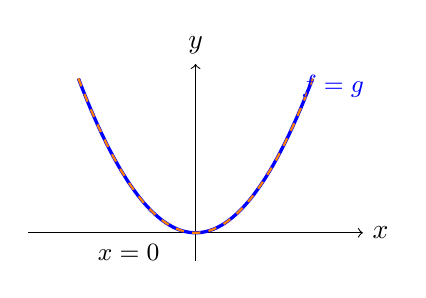
\begin{tikzpicture}[x=.85cm,y=.64cm]
  \draw[->] (-2.5,0)--(2.5,0) node[right] {$x$};
  \draw[->] (0,-.55)--(0,3.35) node[above] {$y$};
  \draw[blue,very thick,domain=-1.75:1.75,samples=60] plot (\x,{\x*\x});
  \draw[orange,dashed,thick,domain=-1.75:1.75,samples=60] plot (\x,{\x*\x});
  \node[blue,font=\small] at (2.05,2.9) {$f=g$};
  \node[font=\small] at (-1.0,-.4) {$x=0$};
\end{tikzpicture}
\end{center}
\textbf{题目：}已知 $f(x)=x^2$。求关于 $y$ 轴翻折后的新函数 $g$，并判断原图自身是否关于 $y$ 轴对称。

\textbf{解：}先用两图相互对称的规则，
\[g(x)=f(-x)=(-x)^2=x^2.\]
再比较：$g(x)=f(x)$，而两函数定义域都为 $\mathbb R$。所以\textbf{两图镜像完全重合，$f$ 自身关于 $y$ 轴对称}。

\textbf{解题提醒：}不要把“$y=f(x)$ 与 $y=f(-x)$ 关于 $y$ 轴对称”当成最终答案；题目还问原图是否\textbf{自身}对称，必须再比较 $g$ 与 $f$。
\end{examplebox}
\clearpage
\begin{examplebox}
\textbf{例 7｜同样是关于 $y$ 轴翻折，却变成另一张图（相互对称）}
\begin{center}
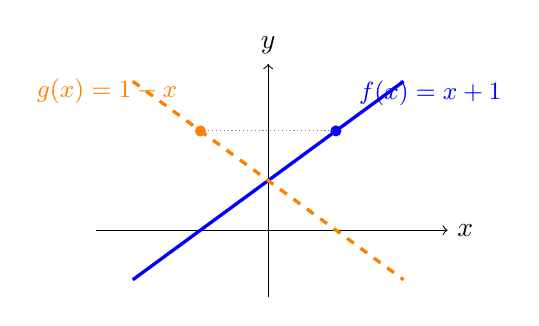
\begin{tikzpicture}[x=.86cm,y=.63cm]
  \draw[->] (-2.55,0)--(2.65,0) node[right] {$x$};
  \draw[->] (0,-1.35)--(0,3.35) node[above] {$y$};
  \draw[blue,very thick] (-2,-1)--(2,3);
  \draw[orange,dashed,very thick] (-2,3)--(2,-1);
  \fill[blue] (1,2) circle (2pt);
  \fill[orange] (-1,2) circle (2pt);
  \draw[gray,densely dotted] (-1,2)--(1,2);
  \node[blue,anchor=west,font=\small] at (1.2,2.75) {$f(x)=x+1$};
  \node[orange,anchor=east,font=\small] at (-1.2,2.8) {$g(x)=1-x$};
\end{tikzpicture}
\end{center}
\textbf{题目：}已知 $f(x)=x+1$。求关于 $y$ 轴翻折后的 $g$；判断“两图相互对称”和“$f$ 自身对称”哪个说法成立。

\textbf{解：}先求镜像：
\[g(x)=f(-x)=1-x.\]
原图的点 $(1,2)$ 对应新图的点 $(-1,2)$，故\textbf{$f$、$g$ 的两幅完整图像关于 $y$ 轴相互对称}。
但 $f(1)=2$，$f(-1)=0$，原函数左右两侧的高度不相等，所以\textbf{$f$ 自身不关于 $y$ 轴对称}。

\textbf{最快判断：}同样套 $g(x)=f(-x)$，只有检查 $g=f$ 通过时，才能再说\textbf{自身对称}。
\end{examplebox}
